
\documentclass{sig-alternate-05-2015}
\usepackage{textcomp}

\begin{document}

% Copyright
\setcopyright{acmcopyright}
%\setcopyright{acmlicensed}
%\setcopyright{rightsretained}
%\setcopyright{usgov}
%\setcopyright{usgovmixed}
%\setcopyright{cagov}
%\setcopyright{cagovmixed}


% DOI
\doi{December 12, 2016}

% ISBN
%\isbn{Fall 2016 UW Madison}

%Conference
\conferenceinfo{CS838 Fall 2016}{University of Wisconsin-Madison}

%\acmPrice{\$15.00}

%
% --- Author Metadata here ---
%\conferenceinfo{WOODSTOCK}{'97 El Paso, Texas USA}
%\CopyrightYear{2007} % Allows default copyright year (20XX) to be over-ridden - IF NEED BE.
%\crdata{0-12345-67-8/90/01}  % Allows default copyright data (0-89791-88-6/97/05) to be over-ridden - IF NEED BE.
% --- End of Author Metadata ---

\title{Measuring and Improvig Geo Distributed Storage}
\subtitle{CS838 Fall 2016 Project Report}
%
% You need the command \numberofauthors to handle the 'placement
% and alignment' of the authors beneath the title.
%
% For aesthetic reasons, we recommend 'three authors at a time'
% i.e. three 'name/affiliation blocks' be placed beneath the title.
%
% NOTE: You are NOT restricted in how many 'rows' of
% "name/affiliations" may appear. We just ask that you restrict
% the number of 'columns' to three.
%
% Because of the available 'opening page real-estate'
% we ask you to refrain from putting more than six authors
% (two rows with three columns) beneath the article title.
% More than six makes the first-page appear very cluttered indeed.
%
% Use the \alignauthor commands to handle the names
% and affiliations for an 'aesthetic maximum' of six authors.
% Add names, affiliations, addresses for
% the seventh etc. author(s) as the argument for the
% \additionalauthors command.
% These 'additional authors' will be output/set for you
% without further effort on your part as the last section in
% the body of your article BEFORE References or any Appendices.

\numberofauthors{2} %  in this sample file, there are a *total*
% of EIGHT authors. SIX appear on the 'first-page' (for formatting
% reasons) and the remaining two appear in the \additionalauthors section.
%
\author{
% You can go ahead and credit any number of authors here,
% e.g. one 'row of three' or two rows (consisting of one row of three
% and a second row of one, two or three).
%
% The command \alignauthor (no curly braces needed) should
% precede each author name, affiliation/snail-mail address and
% e-mail address. Additionally, tag each line of
% affiliation/address with \affaddr, and tag the
% e-mail address with \email.
%
% 1st. author
\alignauthor
Karan Bavishi \\
       \affaddr{UW Madison}\\
% 2nd. author
\alignauthor
Hasnain Ali Pirzada\\
\affaddr{UW Madison}\\
% 3rd. author
}


\maketitle
\section{Problem Statement}
HDFS and other distributed file systems are designed to work in a single data center and do not scale well to geo distributed environment. The primary reason for this is the heterogeneity in speeds of the the inter and intra datacenter links and the fact that the file system itself is unaware of the thin links that connect multiple geo locations. One major way to overcome these problems is to use Erasure Coding instead of replication since erasure coding produces much less amount of data compared to replication and as a result the network and storage overheads are reduced. To solve these problems our goal in this project was two fold. Our first target was to quantify and analyse the performance degradation of HDFS (both replication and erasure coding based) running geo distributedly. Depending upon our findings of this, our second major goal was to reduce the impact of thin WAN links on the performance of geo distributed HDFS. We achieved these goals by first benchmarking both HDFS and HDFS Erasure Coding (HDFS-EC) running geo distributedly and compared their performance with the same system running in a single datacenter. In the second phase of the project we modified HDFS-EC and used greedy heuristics to make it WAN aware in both its reads and writes.

%
\printccsdesc


\keywords{HDFS; Erasure Coding; Geo Distributed Storage}

\section{System Set up}
The first part of our project was to quantify the degradation in HDFS and HDFS-EC performance in Geo Distributed (GD) settings. To do this, we set up a cluster of machines placed in different geo locations , with HDFS running on top of them. We needed to chose the number of machines and the replication factor in such a way that at least one replica is guaranteed to be on a datanode in another DC so that the WAN links are brought into play. 

To be able to measure the extent of degradation in GD settings we also needed to run the same set of experiments in a non GD environment. Furthermore, to compare the extent of degradation in replication based scheme vs the erasure coding scheme we needed to run the same set of experiments on HDFS with replication as well as HDFS-EC in both GD and non GD environment. So in total we had four different settings which are described and explained as follows:

\begin{enumerate}
  \item \textbf{HDFS-Replication based} HDFS running with replication factor 3 with three datanodes in Wisc CloudLab. This is the base case for measuring  and compare the GD degradation in replication based HDFS. There is no remote node since there is just one datacenter.  
	\item \textbf{HDFS-Replica-GD} HDFS running with replication factor 3 with two datanodes in Wisconsin CloudLab and one datanode in Clemson. A replication factor of 3 here with 2 datanodes in Wisconsin and 1 in Clemson ensure that one replica of each block is located remotely.
	\item \textbf{HDFS-EC} HDFS running with erasure coding scheme Reed-Solomon (3,2) with five datanodes in Wisc CloudLab. HDFS-EC fork that we used\cite{hdfsec} required at least n + r datanodes in the cluster while using  RS(n,r) erasure coding scheme. This is done to ensure that cells of a data stripe are well distributed across the cluster since the number of failures that can be tolerated here is equal to r i.e., 2 in this case. A good distribution of the stripe cells ensures better fault tolerance.  Hence, for this configuration we require 3 + 2 = 5 datanodes. All of them are in Wiscnosin.
	\item \textbf{HDFS-EC-GD} HDFS running with erasure coding scheme Reed-Solomon (3,2) with four datanodes in Wisc CloudLab and one datanode in Clemson. The reason for choosing 5 nodes in total is same as the above one. However, now four of the five datanodes are in Wisconsin and one is in Clemson forcing every write to involve the WAN. 
  \end{enumerate}
The WAN speed for all the above configurations is measured to be around 1 Gbps while the intra DC links are all 10 Gbps. This high difference in the two link speeds allows us to more realistically observe the effect of WAN link degradation. We rigorously evaluated all the HDFS variants described using the TestDFSIO workloads. The details are in the experiments and results section. 

\section{System Design \& Implementation}
Drawing insights from the results (which we describe and explain in the results section) of our performance benchmarking of HDFS in GD settings (both replicationa and EC based)  we implemented WAN awareness in HDFS-EC and tuned both the read and write pipelines to take WAN into account while deciding on the datanodes for read/write for the HDFS client. 
\subsection{WAN awareness for HDFS-EC Reads Using Greedy Heuristic}
We build the motivation for WAN aware HDFS-EC reads with an example. Let us say we have a file stored in HDFS-EC running atop a cluster which has nodes in two datacenters A and B. The file is stored as a stripe of cells with some cells representing actual data and others representing parity. In one Reed-Solomon(3, 2) group the file has 3 cells of data which would result in a total of 5 cells written in HDFS 3 being the data cells and 2 being the parity cells. Assume that datacenter A has 2 data cell and one parity cell, while datacenter B has 1 data cell and one parity cell. Now, theere is an HDFS-EC client in datacenter A who wants to read a file.  The default policy is to read all the data cells. The parity cells are only read when the data cell is unavailable because of the high computation cost of reconstructing the data from parity.

In a single data center circumstances, this makes sense because the computation cost is very likely to exceed the network cost that is paid to read a data cells from a remote node.  However, in a GD cluster, this may not be true because the WAN link is much thinner than the intra DC links. Our insight was that it might be faster to actually read 2 data cells and 1 parity cell locally (i.e., from datacenter A) and reconstruct all the three datacells in datacenter A avoiding the WAN link altogether.

To achieve this, we associate costs with every network link. The cost for a WAN link is much higher than the cost for inter DC links. We also associate cost with the reconstruction of data cells using 1 or more parity cells. In our current model, these costs are static and hardcoded at the beginning. At the time of reading, the client picks the r cells with the minimum cost. Note that if a parity cell is chosen, it implies that the link cost for reading this cell plus the computation cost of reconstructing the data using this parity cell and other data cells is still lower than the link cost of the next avaialble data cell. So in the above example since the WAN cost is much higher the client would read 2 data cells and 1 parity cell from datacenter A and use these to reconstruct the 3rd data cell.

\subsection{WAN awareness for HDFS-EC Writes Using Greedy Heuristic}
The write policy in HDFS-EC is similar. The namenode selects (r + s) nodes for writing r data cells and the corresponding s parity cells. It then writes these cells in round robin way to these r + s datanodes. This is done to avoid the loss of multiple data cells in case of a datanode failure. However, while choosing the datanodes to store data and parity cells, the namenode can select a datanode in the other datacenter despite having a datanode locally. This would involve the the write to go through a WAN. 

To prevent this situation, we again implement a simple cost model in the HDFS-EC write pipeline. We associate a parameter we call samerackpenalty with every file write. Moreover, we have link costs available between every pair of racks in the topology. Whenever an HDFS-EC client wants to write a file, the namenode sorts the available datanodes according to their distance from the writer. Now, for each block to be written, it picks the datanode with the minimum cost and remembers the rack from which this datanode was picked. When choosing a datanode for the next block to be written it picks the datanode with the minimum cost with the added constraint that if a datanode has already been chosen from the same rack the total cost of this node becomes linkcost+samerackpenalty and if this total cost is still the minimum of the cost of all the available data nodes this  datanode is chosen. This way, for any subsequent iterations, the cost of this datanode would be (linkcost + n * samerackpenalty) where n is the number of times a datanode from this rack has been chosen for this client. 

\textbf{How does this scheme help?}

This method of selecting the datanodes for writes has a direct affect on the WAN usage. Since the link cost of any datanode in datacenter B is always much higher, the namenode will select the write locations which are closer to the writer reducing the WAN usage. A side effect of this would be that the data would be aggregated near the producers (at least for small files). For large enough files however, the datanodes in the remote datacenter would eventually be selected since penalty for a given rack increases linearly with the number of cells that have already been written in the same rack so at some point selecting a rack in the same datacenter would have more cost than writing to the remote one. 

\section{Experiments \& Results}

Our experiments and results for this project are divided into two parts. In the first part we describe and explain the the benchmarking experiments we performed to measure the degradation of performance of HDFS and HDFS-EC in GD settings. In the second part we discuss the results of WAN aware HDFS-EC that we implemented. Note that all the results we report here are averaged over 10 runs. %For the sake of fair comparison we drop the buffer cache between runs. 	
\subsection{Benchmarking Results}
We run TestDFSIO for four different kinds of measurements. Small file reads, small file writes, large file reads and large file writes and report the results for each kind of test case. Running the same tests for two different size of  files gives us additional insights on how the read and writes of geo distributed HDFS and HDFS-EC are affected by the file size. We discuss and explain all of our observations below. 

For our HDFS performance measurements we run the TestDFSIO benchmark on a Hadoop cluster and measure HDFS read / write throughput of the system. In case of geo-distributed cluster we also measure the total WAN usage. 

\begin{table}
\centering
\caption{Benchmarking Read/Write Throughput (MB/s)}
\label{tput:table}
\begin{tabular}{|c|c|c|c|l|} \hline
Test&Replica&Replica-GD&EC&EC-GD\\ \hline
Small file reads&456.357&456.578&322.664&84.186\\ \hline
Large file reads&748.012&739.626&635.916&174.667\\ \hline
Small file writes&145.071&3.008&116.404&8.523\\ \hline
Large file writes&186.138&3.03&150.258 & 9.05 \\

\hline\end{tabular}
\end{table}
\begin{table}
\centering

\begin{tabular}{|c|c|c|l|} \hline
Test&Replica-GD&EC-GD\\ \hline
Small file reads&2.428&26.058\\ \hline
Large file reads&3.221&381.518\\ \hline
Small file writes&74.135&26.244\\ \hline
Large file writes&1150.637&385.063 \\

\hline\end{tabular}
\caption{WAN usage (MB)}
\label{wan:table}
\end{table}

\textbf{Read/Write Throughput} \\

Table \ref{tput:table} shows the read and write throughput obtained in all the four settings. EC reads worse than replica reads - The read throughput in HDFS-replica is significantly better because in order to read one HDFS block, we can simply fetch the data-local block. However in HDFS-EC with the Reed-Solomon (3,2) encoding scheme, we have to fetch 3 data stripes from different locations in order to read one block (note that a data stripe unit is not equal to an HDFS block). 
EC reads impacted more by GD clusters - The impact of running in geo-distributed clusters is higher on reads in HDFS-EC than on HDFS-replica. This is because in HDFS-EC, all the data stripes (including the one in another DC) have to be fetched to read one block. In HDFS-replica, the reads avoid using the WAN link altogether by picking the closest replica in the same DC.
EC writes worse than replica writes - This is because the parity stripes have to be computed in HDFS-EC before it can be written to the disk and therefore takes more time.
Replica writes impacted more in GD clusters - The impact of running in geo-distributed clusters is higher on writes in HDFS-replica than on HDFS-EC. \\

\textbf{WAN Usage} \\

Table \ref{wan:table} shows the results of WAN usage for all HDFS-EC and HDFS replcation for all the four test cases. 

The following observations can be made:
\textbf{Less WAN usage in EC writes:} Erasure coding clearly uses far less WAN bandwidth than the replica scheme. This difference can be explained by two factors:
Storage efficiency - The amount of data stored in HDFS-replica is more than in HDFS-EC. For every X bytes of data, HDFS-replica stores another 2X bytes compared to HDFS-EC which only stores 0.5X extra bytes.


Mismatching testcases - Since the proportion of datanodes in another DC is higher for the HDFS-replica testcase (1/3) compared to that for HDFS-EC (1/5), the amount of data that needs to flow through the WAN link is also lower. To be fair, even if we had say 2 of the 5 datanodes in another DC in HDFS-EC, we expect the WAN usage to be less for EC. The reason for this configuration is explained in the system set up section. 


\textbf{More WAN usage in EC reads} This is because the local replicas are picked in the replica scheme. Hence the WAN usage is very small.  However, in EC some cells of all the logical file blocks are in the Clemson cluster because of the round robin placement of cells across the datanodes. As a result, every read involves reading some cells from the remote node hence the WAN usage is much higher. 

\subsection{WAN Awareness Results}
For our WAN aware HDFS-EC-GD writes the system setup is slightly different. We run the experiments for a total of 6 datanodes now. Five of these datanodes are in Wisconsin while the sixth one is in Clemson. This gives the writer a choice of chosing between either all the 5 Wisconsin nodes or 4 Wisconsin nodes and 1 Clemson node. If we had less than 5 nodes in Wisconsin than it would not be possible to measure if our algorithm is actually saving any WAN writes since each write would be forced to go over the WAN since a minimum of 5 datanodes are required for RS(3, 2) erasure coding.

\begin{figure}

\centering
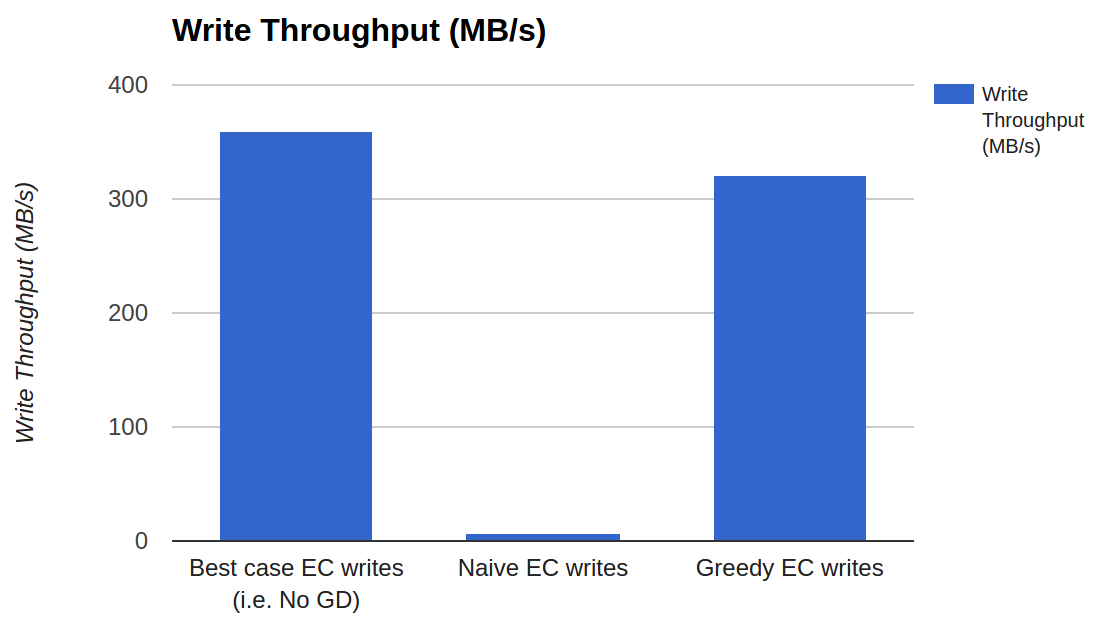
\includegraphics[scale=0.25]{greedy_write_tput.png}
\caption{HDFS-EC write throughput with No-GD (best case), Naive GD and Greedy WAN aware GD}
\label{greedyTput}
\end{figure} 

\begin{figure}
\centering
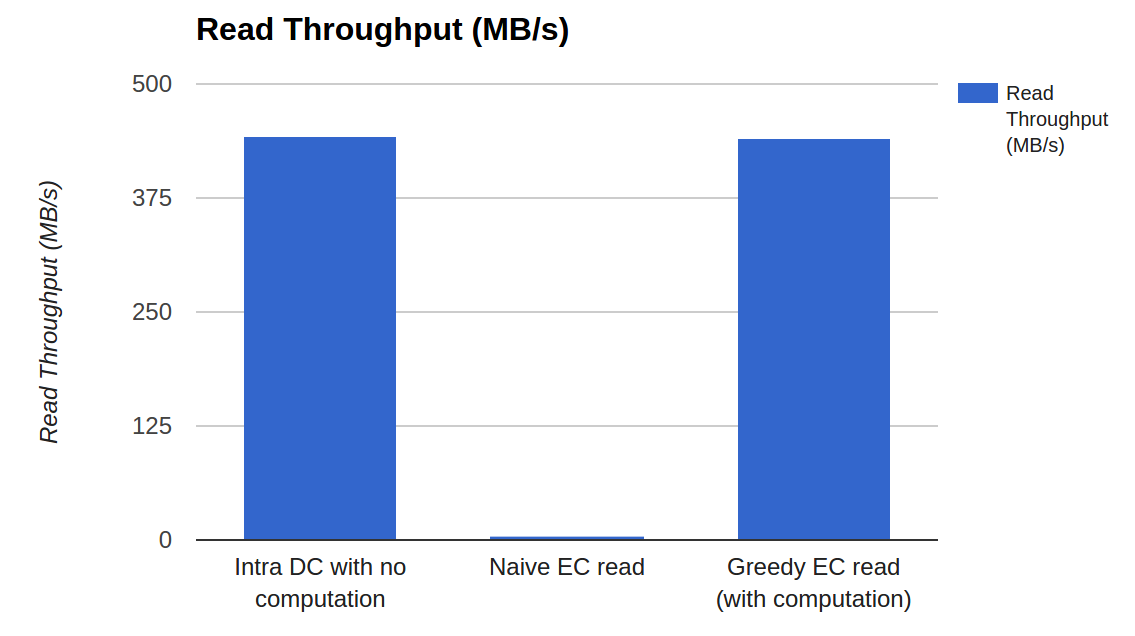
\includegraphics[scale=0.23]{greedy_read_tput.png}
\caption{HDFS-EC Read throughput with No-GD, Naive GD and Greedy WAN aware HDFS-EC-GD}
\label{greedyReadTput}

\end{figure} 

Figure \ref{greedyTput} shows the write throughput for this setting. Naive GD represents the write scenario without using our greedy heuristic to save WAN bandwidth. The best case represents a cluster with all nodes in one datacenter. It acts as a best case comparison point since no WAN link is traversed. In the plot we can see Greedy EC throughput is much higher than the naive EC throughput and is very close to the best case throughput. This is because for the naive write, the namenode selects the datanode in Clemson since it is in a different rack than all the other available nodes. The namenode is unaware that this rack is actually in a different datacenter. As a result,  WAN is used on each write which constrains the write throuput attained. Our greedy write heuristic however has cost for all the links and the cost of the WAN link is much higher than intra DC links. Therefore, the Clemson node is not chosen for writes initially. So, the throuput attained is very close to the best case as WAN is not involved at all. However, after each write in a rack, the rack penalty keeps increasing linearly and eventually writing within the rack at Wisconsin, is more expensive than traversing the WAN and writing to the Clemson datanode. When that happens, WAN is used. As a result, the write throuhput with this greedy write approach is close to but still less than the best case writes (which do not have any WAN to traverse). We can extrapolate that if the file sizes are very large (much larger than the 1 GB we used) this difference would become higher since these WAN writes would be more frequent. 



\begin{figure}

\centering
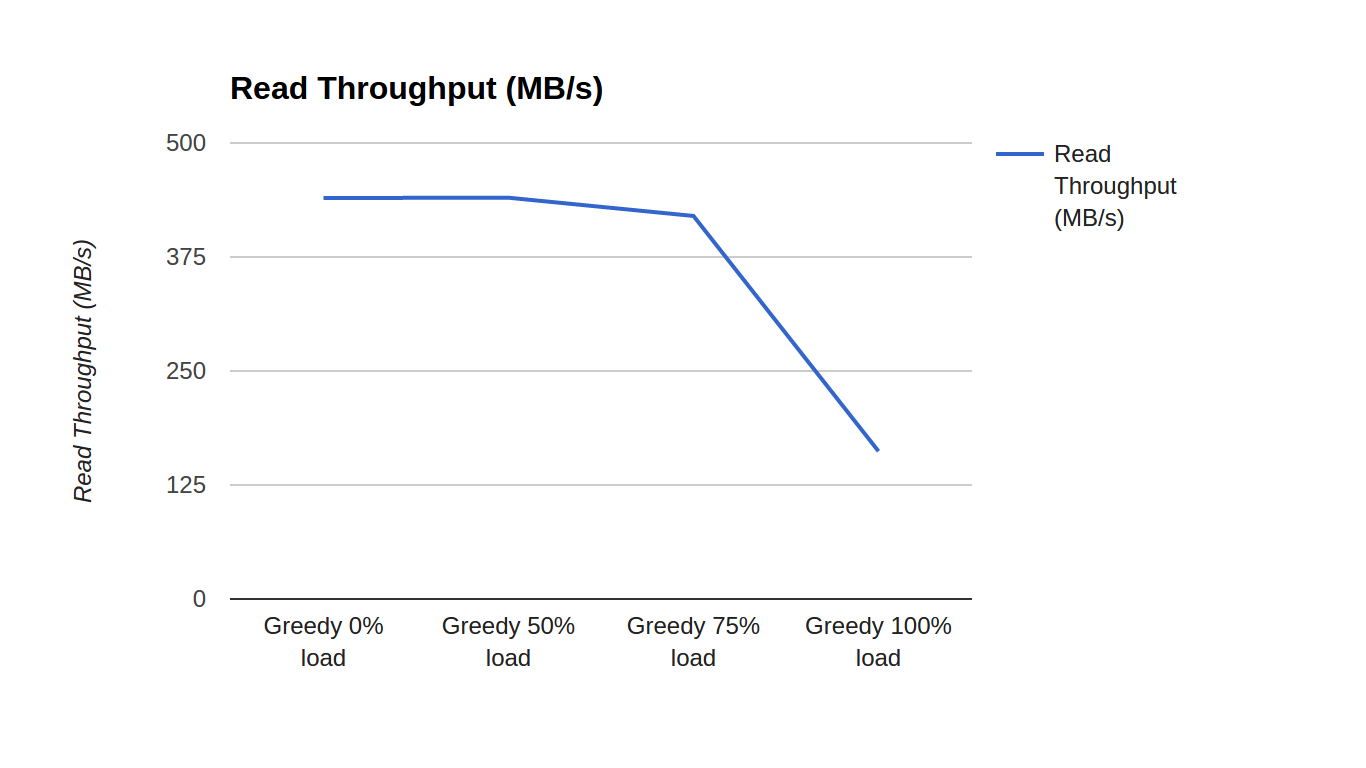
\includegraphics[scale=0.21]{stress.png}
\caption{Read throughput of greedy WAN aware HDFS-EC-GD with varying cpu load}
\label{stress}
\end{figure}
 %This is done because RS(3,2) needs at least five datanodes to spread its cells as described in system setup section. %However, to be able to show that our greedy heuristic for reducing writes over WAN we provide all the 5 nodes in Wisconsin So the 
Figure \ref{greedyReadTput} shows the read throughput achieved through greedy recomputation of the data block using the parity blocks which are avaible locally. To demonstarate the effect of our greedy recomputation we ran the experiments with 4 datanodes in Wisconsin and 1 in Clemson. This would mean that one cell of each stripe in RS(3, 2) is across the WAN. Furthermore, we want to make sure that the cell in Clemson is a data cell and not a parity cell. This would ensure that we actually face the situation where we have the option of either doing a data cell read over the WAN or reconstructing that data cell using the parity cell that is available locally. 

To force HDFS-EC-GD into writing data cells in Clemson we performed our greedy writes with a very high rack penalty. Since, the cells are placed in round robin way and the first 3 cells are the data cells while the next two parity cells, this meant that the datanode for our second cell was always chosen to be in Clemson and since second cell is the data cell we always had a remote data cell.  

Now at the time of read, the naive HDFS-EC read always reads the data cells unless they are unavailble due to datanode failure. %In that case, it informs the namenode of the unavailability (or namenode detects that itself after hearbeat goes missing for an hour) and the reconstruction of the missing cells is quickly done in parallel. 
As a result, it has to fetch one cell from Clemson for every read so the read throughput is extremely low. For our greedy reads however, we just pick R cells which have the least cost out of a total of R + S cells. If all of these R cells are data cells we are done. If some of these are parity cells then we recompute the missing data cells. For data cells, this cost is equal to the static link cost we picked in the beginning. For parity cells, this cost is equal to the link cost plus the computation cost for reconstructing the missing data cell. In this test case, as the WAN link cost is much higher than the computation cost the parity cell is always preferred over the remote data cell as a result WAN is never traversed and instead the missing data cell is always recomputed. Since we had dedicated physical machines for this evaluation, our compute capacity was never a bottleneck and the data cells were reconstructed very fast from the parity cells and the available data cells. As a result, the read troughput is almost equal to the non GD read throuput. 

In a more realistic scenario however, the compute could be a bottleneck so measure the effect of limited compute avaialability, we stress using the linux stress tool to 50\% cpu load 75\% cpu load and 100\% cpu load and measured the trhoughput achieved by our greedy reads scheme. Figure  \ref{stress} shows the effect of cpu load on the read throughput of greedy HDFS-EC-GD reads. Although, this throughput decreases with increasing cpu load, it is still much higher than the reads invovling WAN. 

\section{Discussion}

\subsection{Erasure Coding Properties}

There are various kinds of encoding families that can be used to encode data. These include RS codes, LRC codes and the product codes. Since HDFS-EC used RS encoding we will restrict our discussion to tradeoffs of using different values k and r in RS encoding. According to the coding theory a (k, r) RS code entails the minimum storage overhead among all (k, r) erasure codes that tolerate any r failures \cite{hitchhiker}. Moreover, RS codes can be constructed with arbitrary values of k and r depending upon the system at hand \cite{hitchhiker}. These two properties make RS codes very attractive for use in large scale storage systems. 


The choice of the parameters k and r for any particular system determines the storage overhead and recovery cost for the system. In general achieving lower storage overhead increases the recovery cost of the system and vice versa. For Example, an RS(10, 4) system has a 1.4x overhead compared to 1.5x for RS (6, 3). However, in case of an unavailable datablock RS (10, 4) has to read 10 blocks while RS (6, 3) only needs to read 6.This trend can be generalized for any possible values or k and r. 



\subsection{Significance of Storage Unit to Encode}

The storage unit to be encoded is determined by the layout of the file system. This layout can be contiguous or striped. In contiguous layout a logical block of the file system is mapped directly to a datanode. Reading that block merely involves contacting that particular datanode and doing one I/O.  In striped block layout however, a single logical block in the file system is broken down into small cells and these cells are then mapped to the available datanodes in a round robin manner. Therefore, in the striped layout case, reading a single logical datablock of the file system involves doing I/O with all the datanodes that store the cells of that block. 

%This however, may not be very suitable for Map-Reduce style applications because data %locality cannot be achieved as most reads would involve multiple remote I/Os.

In the replication based storage, a contiguous layout seems to be an obvious choice as there is no point in paying an extra cost of many remote reads for every read event. However, in Erasure Coded storage, things become a little more interesting. This is because the number of parity blocks computed in RS encoding scheme is always equal to r irrespective of the total number of data blocks in the file \cite{blog}. For example, while using RS (10, 4) if a file consists of just one data block, it will still end up computing and writing 4 parity blocks resulting in a total storage overhead of 400\% which is worse than 3x replication! However, in a striped layout and assuming a cell size of 1 MB and the HDFS data block size of 128MB the same 1 block file would still have a 1.4 x overhead since it will produce about 51 MBs of parity (since the parity is computed for 1 MB stripe cells) compared to 512 MB of parity produced by the contiguous layout for the same 128 MB file. 

Therefore, the type of file system layout directly affects the storage overhead for the erasure coding scheme at hand. This choice of layout in turn is determined the file size distribution on the cluster. Hence, a cluster with many small files is not suitable for erasure coding in the contiguous layout because the storage overhead would be worse than replication. The HDFS-EC alpha release that we used and extended uses a striped layout with 1 MB cell size. 

\section{Future Insights}

Our greedy approaches for chosing datanodes for reads and writes show that they can be effective in reducing the performance degradation of HDFS running in GD settings. The benefits achieved by these schemes are due to the fact that they minimize the use of WAN in the read and write pipeline. For HDFS-EC-GD reads our current model just reads the cells with minimum cost and ignores the other constraints of the system. This may not always be beneficial e.g., in a scenario when WAN link utilization is very low and cpu utilization is very high. It would be interesting to incorporate the cpu utilization of the reader and and the available bandwidth on the inter DC WAN link. Furthermore, having multiple geo locations (unlike only 2 in our evaluation) would make the problem of selecting datanodes more interesting. Our hunch is that cpu and inter DC link utilization can be incorporated as constraints of a linear formulation which can then be used to select the datanode for reading data/parity cells. An HDFS client then periodically solves this formulation in the background to get an estimate of which datanodes to be selected for subsequent reads/writes. 

Scondly, in the current implementation, the HDFS client reconstructs the data cells itself after reading one or more parity cells. This can be improved by performing reconstruction of data cells in parallel. We can have a coordinator node in each geo location and whenever an HDFS-EC-GD client prefers a local parity cell read over a remote data cell read, it can inform the coordinator node to initiate the parallel reconstruction of the data. This reconstruction job would be launched by the Coordinator node similar to a Map-Reduce job making sure that all the decoding workers write their output to the HDFS-EC-GD client node. This can dramatically speed up data reconstruction while also minimizing the effect of contrained cpu of the client itself. 

\section{Related Work}
Erasure coding is increasingly being preferred over replication to provide reliability in distributed file systems since it has a far smaller storage overhead. For example, Reed-Solomon \cite{RS} is a popular family of codes used in Google\textquotesingle s ColossusFS \cite{colossus}, Facebook\textquotesingle s HDFS \cite{hdfs-raid}, and several other storage systems \cite{rethink, hitchhiker, gpfs}
However erasure coding brings with itself higher block recovery costs. Multiple data blocks have to be brought in through the network to recompute one lost data block in erasure coding, whereas the corresponding network cost for in replication is just one block.  Several efforts have been made in trying to reduce the recovery cost by using alternate coding schemes - namely LRCs \cite{azure}, or using piggybacking mechanisms like in Hitchhiker\textquotesingle s \cite{hitchhiker}. One of the aims of our study is to find out how such strategies would need to be modified for a geo-distributed cluster setup. We can have a WAN-aware block picking strategy for block recovery, which will try to pick blocks nearby instead of over the WAN link.
There has also been some recent work on a hybrid storage system HACFS \cite{tale}, which uses two different erasure codes and dynamically adapts to workload changes. It uses a fast code to optimize for recovery performance and a compact code to reduce the storage overhead

\bibliographystyle{abbrv}
\bibliography{sigproc}

  \begin{thebibliography}{1}

  \bibitem{hitchhiker} JRashmi, K. V., et al. "A hitchhiker\textquotesingle s guide to fast and efficient data reconstruction in erasure-coded data centers." ACM SIGCOMM Computer Communication Review. Vol. 44. No. 4. ACM, 2014.

  \bibitem{blog}  http://blog.cloudera.com/blog/2015/09/introduction-to-hdfs-erasure-coding-in-apache-hadoop/
  
  \bibitem{hdfsec} https://hadoop.apache.org/docs/r3.0.0-alpha1/hadoop-project-dist/hadoop-hdfs/HDFSErasureCoding.html

  \bibitem{tale}Xia, Mingyuan, et al. "A tale of two erasure codes in hdfs." 13th USENIX Conference on File and Storage Technologies (FAST 15). 2015.
  
  \bibitem{RS} REED, AND SOLOMON - Polynomial codes over certain finite fields. Journal of the So-ciety for Industrial and Applied Mathematics.
  
  \bibitem{colossus} Colossus, successor to Google File System.
  
  \bibitem{hdfs-raid} Facebook\textquotesingle s erasure coded hadoop distributed file system (HDFS-RAID). 
  
  \bibitem{rethink} KHAN, BURNS, PLANK, PIERCE, AND HUANG - Rethinking erasure codes for
cloud file systems: Minimizing I/O for recovery and degraded reads.

  \bibitem{gpfs} SCHMUCK, AND HASKIN - GPFS: A shared-disk file system for large computing clusters. 
  
  \bibitem{azure} HUANG, SIMITCI, XU, OGUS, CA, IDER, GOPALAN, LI, YEKHANI - Erasure coding in Windows Azure Storage

  \end{thebibliography}



\end{document}
